%% Template for ENG 401 reports
%% by Robin Turner
%% Adapted from the IEEE peer review template

%
% note that the "draftcls" or "draftclsnofoot", not "draft", option
% should be used if it is desired that the figures are to be displayed in
% draft mode.

\documentclass[peerreview]{IEEEtran}
\usepackage{cite} % Tidies up citation numbers.
\usepackage{url} % Provides better formatting of URLs.
\usepackage{booktabs} % Allows the use of \toprule, \midrule and \bottomrule in tables for horizontal lines
\usepackage{graphicx}


\hyphenation{op-tical net-works semi-conduc-tor} % Corrects some bad hyphenation 



\begin{document}
%\begin{titlepage}
% paper title
% can use linebreaks \\ within to get better formatting as desired
\title{Dependence Guided Model Checking}


% author names and affiliations

\author{Sabrina Sayasith, Callie Griffin, and Rodion Podorozhny\\
Smith College. Appalachian State University, and Texas State University\\
}
\date{08/3/17}

% make the title area
\maketitle
\tableofcontents
\listoffigures
%\listoftables
%\end{titlepage}

\IEEEpeerreviewmaketitle
\begin{abstract}
The purpose of this research was to create an algorithm that would do a guided depth-first traversal of a control flow graph. In the current implementation of our algorithm, we have Weiser's algorithm operating on a manually produced control flog graph. It was found that Weiser's algorithm greatly reduced that amount of pathways to go down, because of how much irrelevant code was trimmed away. It also reduced the amount of time it took to do a non deterministic execution of depth first search for each control flow graph. To finish the implementation of our algorithm, we would like to implement a forward slicing algorithm in addition to Weiser’s slicing algorithm for more dependency sets and information to be used in the depth-first search traversal, combine the slicing and verification algorithms into one forward pass of the control flow graph, and get the algorithm working on realistic sized systems. 
\end{abstract}


\section{Introduction}
Model checking is a way to formally verify certain properties in a system, which uses temporal logic formulas and symbolic algorithms. Verification is the process of ensuring that a system will function as intended under all circumstances. It can be difficult for all types of systems, but can be especially difficult for cyber-physical systems(CPS) because CPS have an extra layer of physical constraints and environmental factors to account for. Cyber physical systems are systems that have a seamless integration of both algorithms and physical components. Some examples of CPS are autonomous vehicles, smart grids, and medical monitoring systems. Currently, there are two types of verification that can be used on cyber physical systems: static verification and dynamic verification. Static verification is a type of verification that checks all possible execution paths of a program without actually running the program. While thorough, it is immensely time consuming, and it cannot realistically be used on larger systems. Dynamic verification(also known as testing) is the actual testing of an application by running it.  This type of verification allows for testing under real and simulated conditions, but cannot account for all possible scenarios. The fast and thorough verification of cyber physical systems is important because of our steadily increasing reliance upon cyber physical systems. The failure of cyber physical systems could result in costly, and dangerous, accidents. 

\section{Problem Definition}
Currently, the two types of verification that exist for cyber physical systems have too many negative aspects. Static verification is too time consuming and is impossible to use on a realistic sized system becuase of the large number of paths that could be taken, whereas dynamic verification isn't as thorough as cyber physical systems need. 


% An example of a floating figure using the graphicx package.
% Note that \label must occur AFTER (or within) \caption.
% For figures, \caption should occur after the \includegraphics.
% Note that IEEEtran v1.7 and later has special internal code that
% is designed to preserve the operation of \label within \caption
% even when the captionsoff option is in effect. However, because
% of issues like this, it may be the safest practice to put all your
% \label just after \caption rather than within \caption{}.
%
% Reminder: the "draftcls" or "draftclsnofoot", not "draft", class
% option should be used if it is desired that the figures are to be
% displayed while in draft mode.
% 

\begin{figure}[!h]
\centering
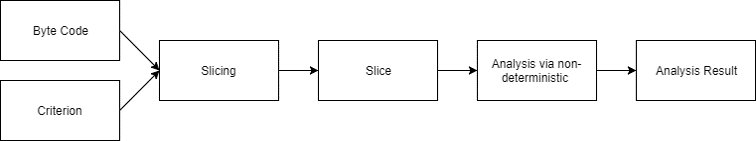
\includegraphics[width=0.8\columnwidth]{ProjectOverview} 
\caption{The overview of our algorithm.}
\label{fig_sim}
\end{figure}

\begin{figure}[!h]
\centering
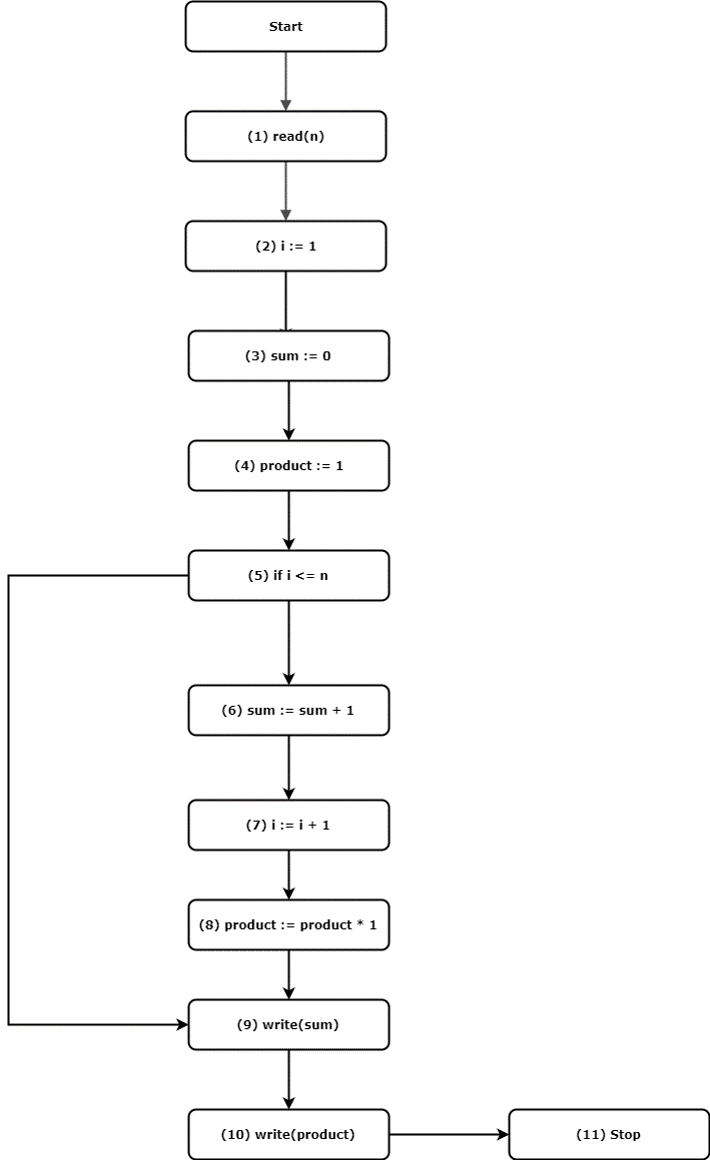
\includegraphics[width=0.8\columnwidth]{CFGBefore} 
\caption{A control flow graph for a program that computes a sum and product with an if statement.}
\label{fig_sim}
\end{figure}

\begin{figure}[!h]
\centering
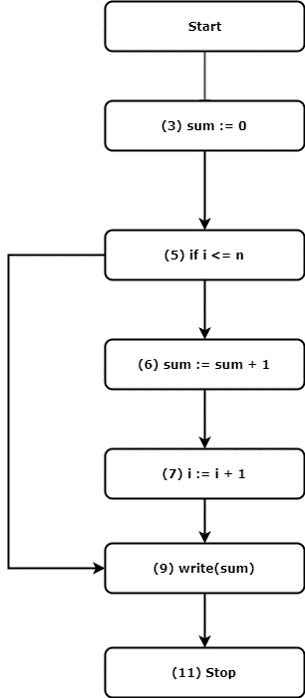
\includegraphics[width=0.8\columnwidth]{CFGAfter} 
\caption{The control flow graph of the program after it has been sliced to only include statements related to the computation of the sum.}
\label{fig_sim}
\end{figure}

% Note that IEEE typically puts floats only at the top, even when this
% results in a large percentage of a column being occupied by floats.
\section{Approach} \label{sec:criteria}
Our approach was to build an Android monitoring system that performed occasional, non-deterministic execution on small pieces of byte code produced by automatic slicing. This monitoring system would use both slicing and non-deterministic execution in one pass that verifies properties and is guided by data and control dependencies. The monitoring verification system would run while the CPS control system functioned.  



\section{Implementation}
Our current prototype is an implementation functioning on a manually created control flow graph. Our implementation of Weiser’s slicing algorithm on the control flow graph limits the number of paths we need to traverse. Weiser’s algorithm chooses the paths based on a stopping point and variables of interest (criterion). We also have a control flow graph creator that creates a CFG for a given program by using the BCEL library to manipulate the byte code of the program.  


\section{Analysis and Interpretation}

	We evaluate the effectiveness of our algorithm against two metrics: the time reduction when traversing the CFG, and the size reduction of the CFG. Time reduction is measured by taking the total time it takes to traverse the unaltered control flow graph and comparing it to the time it takes to traverse the sliced control flow graph. Size reduction is measured by comparing the number of nodes in the original control flow graph to the number of nodes in the sliced control flow graph. -Why did we choose this method of evaluation?-
	We created three different example codes to test our system against. We ran our system through one simple sequential code example, one code example with an if statement, and one code example with a while loop. The timing results of the slicing are given in Figure...



\begin{figure}[!h]
\centering
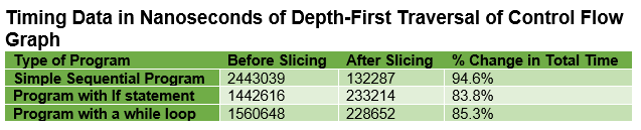
\includegraphics[width=0.8\columnwidth]{SlicingTimes} 
\caption{The time taken for non deterministic execution of depth first search for each control flow graph before and after slicing.}
\label{fig_sim}
\end{figure}

\begin{figure}[!h]
\centering
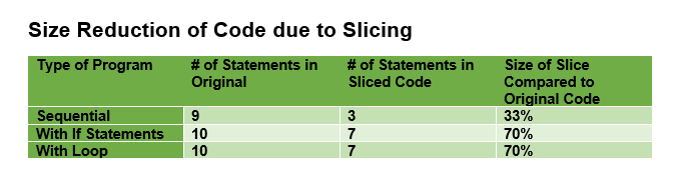
\includegraphics[width=0.8\columnwidth]{SlicedPercentage} 
\caption{The ratio of nodes or statements that remain once sliced.}
\label{fig_sim}
\end{figure}


\section{Conclusions and Recommendations}
	Slicing contributes significantly to reducing the time taken for nondeterministic execution of the control flow graph. The speedup is more pronounced for programs that do not include branch statements(loops and if statements). The reason for this is because if one of the variables contained in the slicing criterion is contained in the REF or DEF sets of one of the statements in the INFL set of one of the branch nodes, then the branch statement must be included in the slice. The required inclusion of the branch statement adds another traversal path and extends the overall traversal time.
	Furthermore, it is unviable to merge a backwards slicing algorithm with forward non-deterministic execution to achieve one single pass of the control flow graph. Our original aim was to have a monitoring system that interrupted a dynamic test scenario with static testing at periodic intervals. This would require the dynamic scenario to execute through the control flow graph from the start to end. However, the algorithm we use, Weiser’s algorithm, requires a backwards execution. In short, we attempt to do depth-first search of the control flow graph that is based on dependency sets and information from Weiser’s algorithm, but we can’t guide the traversal since we are going forwards and do not have the information from Weiser’s algorithm yet.
    	To achieve our goal of one single pass of the control flow graph, work needs to be done on integrating a forward slicing algorithm with our dynamic testing. This will allow for manageable slices of code to be completely explored when...
Once this system is completed, it should be tested on larger or more realistic sized systems. One of the drawbacks of static verification is its runtime. The static verification used in future work should be bounded to limit the runtime, but it still must be ensured that the verification is thorough enough to catch a satisfactory level of bugs and errors. The system should also be tested on example code with bugs and example code without bugs.
-what are some common methods of testing verification systems?-



\begin{thebibliography}{1}
\bibitem{kopka_1999} Binkley, David. “Precise Executable Interprcedural Slices.” ACM Letters on Programming Languages and Systems, Vol. 2, Nos. 1-4, March-December 1993, Pages 31-45. Print.

\bibitem{kopka_1999} "BraceAssertion: Runtime Verification of Cyber-Physical Systems." 2015 IEEE 12th International Conference on Mobile Ad Hoc and Sensor Systems, Mobile Ad Hoc and Sensor Systems (MASS), 2015 IEEE 12th International Conference on, Mobile Ad-Hoc and Sensor Systems (MASS), 2013 IEEE 10th International Conference on (2015): 298. Print. 

\bibitem{kopka_1999} "Formal Verification of Cyber-Physical Automation Systems Modelled with Timed Block Diagrams." 2016 IEEE 25th International Symposium on Industrial Electronics (ISIE), Industrial Electronics (ISIE), 2016 IEEE 25th International Symposium on (2016): 316. Print. 

\bibitem{kopka_1999} Giffhorn, Dennis, et al. “Precise slicing of concurrent programs. An Evaluation of static slicing algorithms for concurrent programs.” Springer Science+Business Media, LLC 2009. 197-234. 

\bibitem{kopka_1999} Jiang, Siyuan, et al.“On the Accuracy of Forward Dynamic Slicing and its Effects on Software Maintenance.” 2014 14th IEEE International Working     Conference on Source Code Analysis and Manipulation: 145. Print.

\bibitem{korel_1994} Korel, Bogdan, et al. “Forward Computation of Dynamic Program Slices.” Master Essay, Department of Computer Science Wayne State University, 1994. 66-79. Print.

\bibitem{krinka_2003} Krinke, Jens. “Contact-Sensitive Slicing of Concurrent Programs.” ESEC/FSE’03, September 1–5, 2003, Helsinki, Finland. 178-187. Print. 

\bibitem{Larsen} Larsen, Loren, et al. “Slicing Object-Oriented Software.” Proceedings of ICSE-18. Department of Computer Science Clemson University. 495-505. Print. 

\bibitem{Matsubara_2002} Matsubara, Masahiro, et al. "Model Checking with Program Slicing Based on Variable Dependence Graphs." Electronic Proceedings in Theoretical Computer Science, Vol 105, Iss Proc.FTSCS 2012, Pp 56-68 (2012) (2012): 56. Print. 

\bibitem{Podgurski_1990} Podgurski, Andy, et al. “A Formal Model of Program Dependencies and Its Implications for Software Testing, Debugging, and Maintenance.” IEEE Transactions on Softwaree Engineering, Vol. 16, NO. 9. September 1990. 965-979. Print. 

\bibitem{Siroky_2015} Siroky, Colin Stuart. Verification of Architectural Constraints on Interaction Protocols among Modules., 2015. Print. 

\bibitem{Su_2015}Su, T. (. 1. )., et al. Combining Symbolic Execution and Model Checking for Data Flow Testing. 1 Vol. IEEE Computer Society, 2015. Print. 

\bibitem{Tip_1995} TIP, F. A Survey of Program Slicing Techniques. 3 Vol. , 1995. Print. 

\bibitem{Weiser_1984} Weiser, Mark. IEEE Transactions on Software Engineering 10.4 (1984): 352-7. Print. 

\bibitem{Willem_2003} Willem, Visser, et al. "Model Checking Programs." Automated Software Engineering.2 (2003): 203. Print.
\end{thebibliography}

% This is a hand-made bibliography. If you want to use a BibTeX file, you're on your own ;-)














\end{document}


